\noindent
\textbf{CHEM 352:
\ifthenelse{\equal{\solutions}{true}}{Examples}{Homework} for chapter 3.}\\

\noindent
1. a) Show that $sp^2$ hybrid orbital $h = \frac{1}{\sqrt{3}}\left( s + \sqrt{2}p_x\right)$ is normalized.
The functions $s$ and $p_x$ denote normalized hydrogenlike atomic orbitals.\\
\phantom{1. }b) Normalize the following molecular orbital $\psi = \psi_{s,A} + \lambda\psi_{s,B}$ where
$\psi_{s,A}$ and $\psi_{s,B}$ are normalized and $\lambda$ is a parameter. Use the notation $S$ for overlap
integral to simplify the result.\\

\ifthenelse{\equal{\solutions}{true}}{% Problem 1/3 solution
\noindent
\underline{Solution:}\\

The lecture notes give: $C_V = \left(\frac{\partial U}{\partial T}\right)_V$. Differentiate this equation with respect to volume:

$$\left(\frac{\partial C_V}{\partial V}\right)_T = \left(\frac{\partial}{\partial V}\left(\frac{\partial U}{\partial T}\right)_V\right)_T = \left(\frac{\partial}{\partial T}\left(\frac{\partial U}{\partial V}\right)_T\right)_V$$

By using the relation given in the problem, we can write this as:

$$\left(\frac{\partial C_V}{\partial V}\right)_T = \left(\frac{\partial}{\partial T}\left(\frac{\partial U}{\partial V}\right)_T\right)_V = \left(\frac{\partial\left(-P + T\left(\partial P / \partial T\right)_V\right)}{\partial T}\right)_V = T\left(\frac{\partial^2 P}{\partial T^2}\right)_V$$

Next we consider the various equations of state:

\begin{itemize}
\item[a)] Ideal gas. $P = nRT / V$ from which the second derivative of pressure (see above) is zero and therefore $\left(\frac{\partial C_V}{\partial V}\right)_T = 0$.

\item[b)] For a van der Waals gas we have: $P = \frac{nRT}{V - nb} - \frac{n^2a}{V^2}$. Differentiation of $P$ with respect to $T$ once just gives $nR / (V - nb)$. This does not depend on $T$ and hence $\left(\frac{\partial C_V}{\partial V}\right)_T = 0$.

\item[c)] Differentiation of $P$ twice with respect to $T$ again gives zero and hence $\left(\frac{\partial C_V}{\partial V}\right)_T = 0$.
\end{itemize}

\hrule\vspace{0.5cm}
}{}

\noindent
2. Consider hydrogen molecule (H(A)--H(B)) with the LCAO-MO orbitals formed from the atomic orbitals $1s_A$ and $1s_B$:

\begin{center}
$1\sigma_g = N_1\left( 1s_A + 1s_B\right)$ and $1\sigma_u^* = N_2\left( 1s_A - 1s_B\right)$
\end{center}

\vspace{-0.5cm}
\phantom{2. }a) Show that the Slater determinant corresponding to the ground state solution is antisymmetric.\\
\phantom{2. }b) One of the excited states of H$_2$ corresponds to the following Slater determinant:

\begin{center}
$
\psi_{MO} = \frac{1}{\sqrt{2}}\begin{vmatrix}
1\sigma_g(1)\alpha(1) & 1\sigma_u^*(1)\alpha(1)\\
1\sigma_g(2)\alpha(2) & 1\sigma_u^*(2)\alpha(2)\\
\end{vmatrix}
$
\end{center}

\noindent
\phantom{2. b) }What electron configuration does this correspond to?\\

\ifthenelse{\equal{\solutions}{true}}{% Problem 2/3 solution
\noindent
\underline{Solution:}\\

By using the result given in the first problem, we can obtain $\left(\frac{\partial U}{\partial V}\right)_T = 0$. The total differential for $dU$ now gives $dU = \left(\frac{\partial U}{\partial T}\right)_VdT$ and hence $dU = C_VdT$. The first law of thermodynamics, $dU = dq + dw$, gives $dq = C_VdT - dw$. Considering $PV$-work, we can write: $dq = C_VdT + P_{ext}dV$. Because the process is reversible, $P_{ext} = P$ and $dq = C_VdT + PdV$. For $dq$ to be exact we should have:

$$\left(\frac{\partial C_V}{\partial V}\right)_T = \left(\frac{\partial P}{\partial T}\right)_V$$

From the first problem we know that the left hand side is zero. The right hand side, however, is not zero:

$\left(\frac{\partial P}{\partial T}\right)_V = \frac{nR}{V - nb} \ne 0$

Thus $dq$ is inexact. For $dq / T$ we have: $\frac{dq}{T} = \frac{C_V}{T}dT + \frac{P}{T}dV$. Now the exactness test gives:

$$\left(\frac{\partial C_V / T}{\partial V}\right)_T = 0\textnormal{ (}T\textnormal{ is constant)}$$
$$\left(\frac{\partial (nR / (V - nb))}{\partial T}\right)_V = 0\textnormal{ (the expression does not depend on }T\textnormal{)}$$

Thus $dq/T$ is exact.

\hrule\vspace{0.5cm}
}{}

\noindent
3. Determine the valence electron configurations and bond orders in the following molecules:
C$_2^+$, C$_2$, C$_2^-$, N$_2^+$, N$_2$, N$_2^-$, O$_2^+$, O$_2$, O$_2^-$. Which of these
molecules are paramagnetic and what are their term symbols?\\

\ifthenelse{\equal{\solutions}{true}}{% Problem 3/3 solution
\noindent
\underline{Solution:}\\

\textbf{Path 1}: First we recall that for an ideal gas $U = \frac{3}{2} nRT$ (see lecture notes). The temperature is constant along this path and thus change in internal energy must be zero. The first law of thermodynamics now states that $\Delta UU = q_{rev} + w_{rev}$ and hence $q_{rev} = -w_{rev}$. Recall the following equation from the lecture notes:

$$w_{rev} = -nRT_1\ln\left(\frac{V_2}{V_1}\right) \Rightarrow q_{rev} = nRT_1\ln\left(\frac{V_2}{V_1}\right)$$

Using the definition of entropy gives:

$$\Delta S = \frac{q_{rev}}{T_1} = nR\ln\left(\frac{V_2}{V_1}\right)$$

\textbf{Path 2}: First consider the first segment from ($P_1$, $V_1$, $T_1$) to ($P_3$, $V_2$, $T_2$). The expansion is adiabatic (i.e. no heat exchange with the surroundings) and hence $q_{rev} = 0$. For this reason the change in entropy is also zero ($\Delta S = q_{rev} / T = 0$). The final temperature in an adiabatic expansion is determined by integrating $C_V\frac{dT}{T} = -nR\frac{dV}{V}$ (see lecture notes):

$$\int\limits_{T_1}^{T_2}\frac{C_V}{T}dT = -nR\int\limits_{V_1}^{V_2}\frac{dV}{V} = -nR\ln\left(\frac{V_2}{V_1}\right)$$

Along the second segment ($P_3$, $V_2$, $T_2$) to ($P_2$, $V_2$, $T_1$), we have a constant volume process. The lecture notes now give $dq_{rev} = C_VdT$. The definition of entropy is $dS = \frac{dq_{ref}}{T}$ and thus:

$$dS = \frac{C_VdT}{T} \Rightarrow \Delta S = \int\limits_{T_2}^{T_1}\frac{C_VdT}{T} = -\int\limits_{T_1}^{T_2}\frac{C_VdT}{T}$$

Comparison of this with the expression determining $T_2$ along the first segment, gives the final result:

$$\Delta S = nR\ln\left(\frac{V_2}{V_1}\right)$$

This is the same result that was obtained along path 1. For a complete proof of exactness, one would have to use the exactness test or consider infinitely many paths (or rather, the exactness test).

\hrule\vspace{0.5cm}
}{}

\noindent
4. Sketch the molecular orbital diagram for B$_2$ molecule by using $1s$, $2s$ and $2p$ atomic orbitals and
all 10 electrons. What is the term symbol?\\

\ifthenelse{\equal{\solutions}{true}}{% Problem 3/4 solution
\noindent
\underline{Solution:}\\

\noindent
The MO diagram is:\\
\noindent
\begin{figure}[h]
\centering
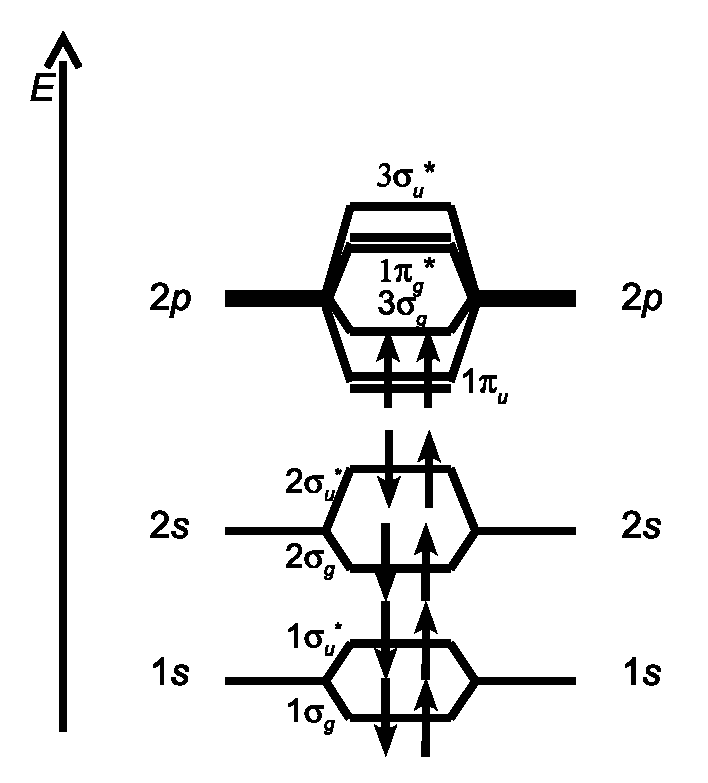
\includegraphics[scale=0.5]{b2mo}
\end{figure}

\noindent
The term symbol is $^3\Sigma_g$.\\

\hrule\vspace{0.5cm}
}{}

\noindent
5. a) Sketch a molecular orbital diagram for XeF molecule and determine the electronic configuration. Would
XeF$^+$ have shorter bond length than XeF?\\
\phantom{5. }b) Construct a molecular orbital diagram for the double bond (4 electrons) in ethene by using
the carbon $sp^2$ hybrid orbitals as basis set. Choose the energy order of the $\sigma$ and $\pi$ orbitals
in such a way that a stable molecule is formed.\\
\phantom{5. }c) Explain why Ne$_2$ molecule is not stable. Why are atoms with the outmost $s$ and $p$ orbitals 
full (e.g. the octet electronic configuration) chemically inert?\\

\ifthenelse{\equal{\solutions}{true}}{% Problem 3/5 solution
\noindent
\underline{Solution:}\\

\noindent
a) XeF is not a homonuclear diatomic molecule. Thus the atomic orbitals 
that form MOs originate from different principal quantum number levels.
The MO diagram is:\\
\newpage
\noindent
\begin{figure}[h]
\centering
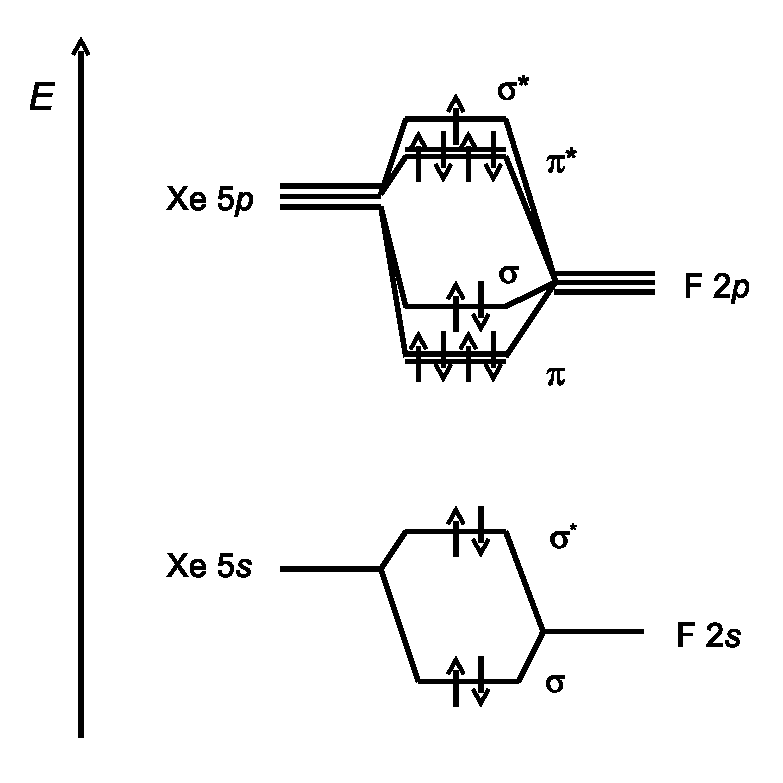
\includegraphics[scale=0.5]{xefmo}
\end{figure}

\noindent
The bond order for XeF is $(8 - 7) / 2 = 0.5$ and for XeF$^+$ $(8 - 6)
/ 2 = 1$. Thus the equilibrium bond length for XeF$^+$ is expected to be
shorter than for XeF.\\

\noindent
b) Consider the MOs of the C=C fragment:
\noindent
\begin{figure}[h]
\centering
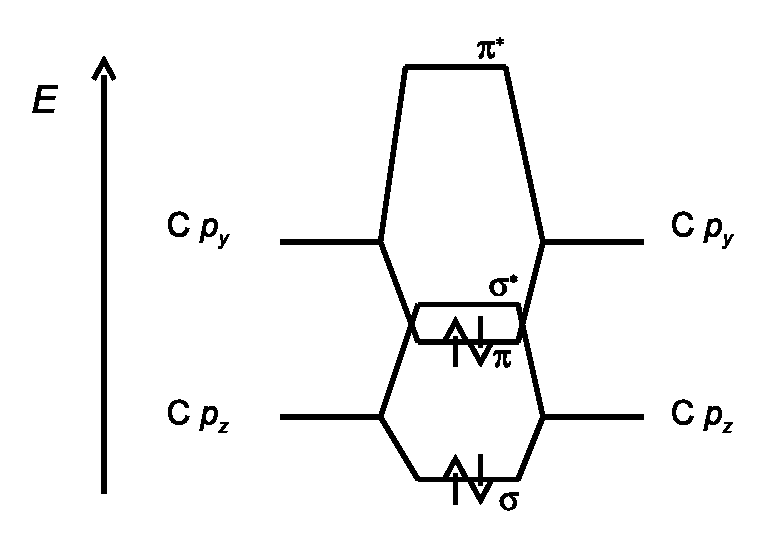
\includegraphics[scale=0.5]{ccmo}
\end{figure}

\noindent
Note that the order of the $\pi$ and $\sigma^*$ orbitals must be as shown
above. If this was not the case, the C=C fragment would not be bound!\\

\noindent
c) All the resulting bonding and antibonding orbitals become fully occupied. 
As antibonding orbitals cause more repulsion than bonding orbitals binding,
the result is no chemical binding. In general, the octet electronic
structure in atoms (e.g. rare gases) tends to lead to efficient population of the antibonding
molecular orbitals and hence they are chemically inert.\\

\hrule\vspace{0.5cm}
}{}

\noindent
6. Use the variational principle to obtain the lowest energy solution to the hydrogen atom Schr\"odinger
equation in spherical coordinates by using the following trial wavefunctions:\\
\phantom{6. }a) $\psi_{trial} = e^{-kr}$ with $k$ as a variational parameter.\\
\phantom{6. }b) $\psi_{trial} = e^{-kr^2}$ with $k$ as a variational parameter.\\
Note that both trial functions depend only on $r$ and the angular terms disappear
from the Laplacian. You may find the following integrals useful:

\begin{center}
$\int_0^\infty x^ne^{-ax}dx = \frac{n!}{a^{n+1}}$\\
$\int_0^\infty x^me^{-ax^2}dx = \frac{\Gamma[(m + 1)/2]}{2a^{(m + 1) / 2}}$\\
$\Gamma[n + 1] = n!$, with $0! = 1$ ($n$ is integer)\\
$\Gamma[n + 1] = n\Gamma[n]$\\
$\Gamma\left[\frac{1}{2}\right] = \sqrt{\pi}$
\end{center}

\ifthenelse{\equal{\solutions}{true}}{% Problem 6/3 solution
\noindent
\underline{Solution:}\\

Tripling of the ideal gas volume ($PV_1 = nRT_1$) leads to $T = P(3V_1) / (nRT)$, which means that the temperature will be three times higher; $T_2 = 3T_1$. Note that pressure is constant.

\begin{itemize}
\item[a)] $q = \int\limits_{T_1}^{T_2}\bar{C}_PdT = \int\limits_{298\textnormal{ K}}^{894\textnormal{ K}}\left(25.895 + 32.999\times 10^{-3}T - 30.46\times 10^{-7}T^2\right)dT = 26.4\textnormal{ kJ mol}^{-1}$.

\item[b)] $w = -P\Delta\bar{V} = -R\Delta T = -\left(8.314\textnormal{ J K}^{-1}\textnormal{ mol}^{-1}\right)\times\left(596\textnormal{ K}\right) = -4.96\textnormal{ kJ mol}$.

\item[c)] Because pressure is constant, we have $\Delta\bar{H} = q_P = 21.4\textnormal{ kJ mol}^{-1}$.

\item[d)] $\Delta\bar{U} = q + w = \left(26.4 - 4.96\right)\textnormal{ kJ mol}^{-1} = 21.4\textnormal{ kJ mol}^{-1}$.

\item[e)] $\Delta\bar{S} = \int\limits_{T_1}^{T_2}\frac{C_P}{T}dT = \int\limits_{298\textnormal{ K}}^{894\textnormal{ K}}\left(\frac{25.895}{T} + 32.999\times 10^{-3} - 30.46\times 10^{-7}T\right)dT = 46.99\textnormal{ kJ K}^{-1}\textnormal{ mol}^{-1}$.

\end{itemize}

\hrule\vspace{0.5cm}
}{}

\noindent
7. Calculate the $\pi$ orbitals of allyl radical (corresponding to localized structure 
$\overset{\textnormal{.}}{\textnormal{CH}_2}$--C=CH$_2$, however, assume delocalization in your calculation)
by using the H\"uckel theory.\\
a) What is the wavelength of the LUMO $\leftarrow$ HOMO electronic transition when $\beta = -22,000$ cm$^{-1}$?\\
b) Calculate the charge densities and bond orders from the H\"uckel wavefunction. Definitions for these
observables are given below:\\

\noindent
\underline{Electron density on atom $i$:}

\begin{center}
$$\rho(i) = \sum_{j = 1}^{N_{MO}} |c_i^j|^2n_j$$
\end{center}

\noindent
where $n_j$ is the number of electrons on orbital $j$ and $c_i^j$ is the H\"uckel MO coefficient of the basis
function centered on atom $i$ for orbital $j$. The summation runs over the occupied orbitals.\\

\noindent
\underline{Bond order between atoms $i$ and $j$:}

\begin{center}
$$\textnormal{bond order} = \sum_{k = 1}^{N_{MO}} c_i^k c_j^k n_k$$
\end{center}

\noindent
where the symbols are defined as above.\\

\ifthenelse{\equal{\solutions}{true}}{% Problem 3/7 solution
\noindent
\underline{Solution:}\\

\noindent
First we construct the secular equation (matrix form) corresponding to the 
H\"uckel approximation:\\

$$\begin{pmatrix}
\alpha - E & \beta & 0\\
\beta & \alpha - E & \beta\\
0 & \beta & \alpha - E\\
\end{pmatrix}
\begin{pmatrix}
c_1\\
c_2\\
c_3\\
\end{pmatrix}
= 0$$

\noindent
Denote $x = (\alpha - E) / \beta$ and recall this set of equations
has a non-trivial solution only if the corresponding determinant is zero:

$$\begin{vmatrix}
x & 1 & 0\\
1 & x & 1\\
0 & 1 & x\\
\end{vmatrix}
= 0$$

\noindent
By expanding this determinant, we get:

$$x(x^2 - 1) - x = x^3 - 2x = x(x^2 - 2) = 0 \Rightarrow x =
\left\{
\begin{matrix}
0\\
+\sqrt{2}\\
-\sqrt{2}\\
\end{matrix}
\right.
$$

$$\Rightarrow E = \left\{\begin{matrix}
\alpha\\
\alpha - \sqrt{2}\beta\\
\alpha + \sqrt{2}\beta\\
\end{matrix}\right.
$$

\noindent
Thus we have the following energetics for the orbitals:

\begin{figure}[h]
\centering
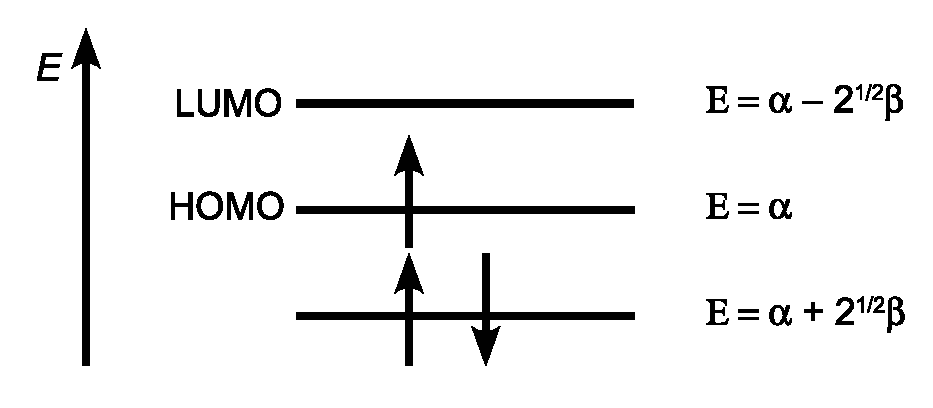
\includegraphics[scale=0.4]{huckelmo}
\end{figure}

\noindent
a) The energy difference between HOMO and LUMO orbitals is:

$$\Delta E = E_\textnormal{LUMO} - E_\textnormal{HOMO} = \alpha 
- \sqrt{2}\beta - \alpha = -\sqrt{2}\beta = -\sqrt{2}\times (-22,000
\textnormal{cm}^{-1})$$

$$\rightarrow \Delta E = 3.86 \textnormal{eV}~(320\textnormal{~nm})$$

\noindent
b) Next we calculate the coefficients $c_1, c_2$ and $c_3$ for the lowest
energy orbital:

\noindent
Here $E = (\alpha\pm\sqrt{2}\beta)$, which with $(\alpha - E)c_1 + \beta c_2 = 0$
gives $c_2 = \pm\sqrt{2}c_1$. Exactly the same way, equation
$\beta c_2 + (\alpha - E)c_3 = 0$ gives $c_2 = \pm\sqrt{2}c_3$.
Finally, normalization gives:
$c_1^2 + c_2^2 + c_3^2 = 1$ $\Rightarrow c_1^2 + (\pm\sqrt{2}c_1)^2
+ c_1^2 = 4c_1^2 \Rightarrow c_1 = \frac{1}{2}$ and by considering
$c_3$ the same way, we also get $c_3 = \frac{1}{2}$.\\

\noindent
Thus we have:

$$E = \alpha + \sqrt{2}\beta~\textnormal{with}~c_1 = \frac{1}{2},
c_2 = \frac{1}{\sqrt{2}}, c_3 = \frac{1}{2}$$
$$E = \alpha - \sqrt{2}\beta~\textnormal{with}~c_1 = \frac{1}{2},
c_2 = -\frac{1}{\sqrt{2}}, c_3 = \frac{1}{2}$$

\noindent
For $E = \alpha$, we have: $c_1 = \frac{1}{\sqrt{2}}, c_2 = 0, c_3 
= -\frac{1}{\sqrt{2}}$.\\

\noindent
The electron density on atom 1 can be obtained by squaring the atomic
basis function coefficients and weighing this by the number of electrons
on that orbital:\\

\noindent
Atom 1 ($i = 1$): $\sum_{j=1}^{3}|c_i^j|^2n_j = 
\left(\frac{1}{2}\right)^2\times 2 + \left(\frac{1}{\sqrt{2}}\right)^2
\times 1 + \left(\frac{1}{2}\right)^2\times 0 = 1$.\\
Atom 2 ($i = 2$): $\sum_{j=1}^{3}|c_i^j|^2n_j = 
\left(\frac{1}{\sqrt{2}}\right)^2\times 2 + 0^2
\times 1 + \left(-\frac{1}{\sqrt{2}}\right)^2\times 0 = 1$.\\
Atom 3 ($i = 3$): $\sum_{j=1}^{3}|c_i^j|^2n_j = 
\left(\frac{1}{2}\right)^2\times 2 + \left(-\frac{1}{\sqrt{2}}\right)^2
\times 1 + \left(\frac{1}{2}\right)^2\times 0 = 1$.\\

\noindent
The total charge (three $\pi$ electrons) is distributed evely to all three
atoms and therefore the partial charges on carbon atoms are equal.\\

\noindent
The bond orders can be valuated as follows:\\

\noindent
Bond between atoms 1 and 2 ($i = 1$ and $j = 2$):\\
$$\sum_{k=1}^{N_{MO}}c_i^k c_j^k n_k = 
\left(\frac{1}{2}\right)\left(\frac{1}{\sqrt{2}}\right)\times
2 + \left(\frac{1}{\sqrt{2}}\right)\times 0\times 1 
+ \left(\frac{1}{2}\right)\left(-\frac{1}{\sqrt{2}}\right)\times 0 
= \frac{1}{\sqrt{2}}$$
Bond between atoms 2 and 3 ($i = 2$ and $j = 3$):\\
$$\sum_{k=1}^{N_{MO}}c_i^k c_j^k n_k = 
\left(\frac{1}{\sqrt{2}}\right)\left(\frac{1}{2}\right)\times
2 + 0\times\left(-\frac{1}{\sqrt{2}}\right)\times 1
+ \left(-\frac{1}{\sqrt{2}}\right)\left(\frac{1}{2}\right)\times 0 
= \frac{1}{\sqrt{2}}$$

\noindent
The bond order is less than one ($\approx 0.707$), which indicates that
the bond is not very strong.\\

\hrule\vspace{0.5cm}
}{}
